\chapter{Metodología de desarrollo}
En este capítulo se explicará la metodología de desarrollo escogida, así como los hechos que motivaron dicha decisión y como se ha aplicado le metodología a nuestro proyecto concreto.
\section{Metodologías ágiles}
Los principales rasgos de una metodología ágil serían los siguientes:
\begin{itemize}
\item Todos los objetivos, fechas límite, decisiones... han de girar en torno al equipo de desarrollo. Las personas serán el centro del proceso y se configurará el entorno según sus necesidades.
\item Se priorizará crear software que funcione correctamente frente a una documentación demasiado detallada.
\item La comunicación con el cliente ha de ser continua y periódica durante todo el proceso, evitando contratos iniciales y una pérdida total de contacto hasta la fecha de entrega.
\item En el desarrollo de software en muy común que surjan imprevistos, es importante tener la capacidad de adaptarse a ellos rápidamente.
\end{itemize}
La localización en interiores es una disciplina cuyas bases no están demasiado asentadas, así que debemos dejar las puertas abiertas a cambios, como por ejemplo nuevas tecnologías o técnicas de obtención de la localización. Una forma inteligente de realizar un proyecto de este tipo, es tratar como una caja negra la obtención de las coordenadas, siendo indiferente para la aplicación como se obtengan. Da igual que sea mediante \textit{GPS}, con la \textit{API} de \textit{Situm} o con cualquier otro servicio. De esta manera, el día de mañana podríamos adaptar el proyecto de manera cómoda a una nueva tecnología, permitiendo a la aplicación evolucionar y no dejándola atrasada por miedo a realizar gran cantidad de cambios.
\subsection*{\textit{SCRUM}}
\textit{Scrum} es una metodología ágil de desarrollo software, está diseñada para equipos de 3 a 9 desarrolladores que dividen el trabajo en iteraciones, llamadas \textit{sprints}. La duración de estos intervalos suele ser de menos de un mes, y suelen realizarse reuniones cortas diarias para analizar el curso que sigue el proyecto.
Cada una de estas iteraciones tiene que proporcionar un resultado completamente funcional, cada una de ellas será una versión del producto final cada vez más avanzada. El proceso completo sigue las siguientes fases:
\begin{enumerate}
\item \label{fase1scrum} primero de todo será una reunión con el cliente para crear una lista de requisitos ordenados por su prioridad, dependiendo del beneficio y del coste de los mismos. Esta lista se elabora con el cliente.
\item \label{fase2scrum} A partir de la lista de requisitos inicial, se selecciona un subconjunto de los mismos que conformarán la siguiente iteración.
\item Se llevan a cabo reuniones periódicas, estas sin el cliente, para poder reaccionar rápidamente ante cualquier problema o requisito que vaya surgiendo a lo largo del desarrollo.
\item El último día de la iteración se lleva a cabo otra reunión, en la cual, sí que se encuentra el cliente. Aquí se analizará el trabajo realizado y los problemas surgidos durante el desarrollo, para que no se vuelvan a repetir en los siguiente sprints.
\item Finalmente, hay que garantizar que el producto que se entrega al cliente sea un software completamente funcional. Si se desea continuar desarrollando más sprints, se repite el proceso desde la fase \ref{fase2scrum}.
\end{enumerate}
\section{Adaptación a nuestro proyecto}
Se ha elegido esta metodología porque las características del equipo de desarrollo son muy diferentes al de una empresa real. La plantilla de programadores consta de un solo integrante y el rol de cliente se jugó a partes iguales por el tutor y por el alumno. Ya que ambos propusieron nuevas metas y objetivos a medida que avanzaba el proyecto, y además, no sólo se realizaron reuniones con el cliente al comienzo y al final de cada \textit{Sprint}, sino que fueron más numerosas.
\subsection*{Roles}
Aquí explicaremos los principales roles de una metodología \textit{SCRUM} y quien los ha representado en este proyecto.
\subsection*{Desarrollo}
\begin{itemize}
\item \textbf{El cliente:} Es el que añade, elimina o prioriza requisitos. Este rol lo ha desarrollado el director del proyecto pero como se comenta anteriormente, es este caso en particular, muchos requisitos también fueron diseñados por el alumno.
Conformarán el total de requisitos que tendrá el proyecto, lo que se llama \textit{Product Backlog}, más tarde, cuando se creen los \textit{sprints}, se hará un estudio de las prioridades de cada uno de estos requisitos y se crearán subconjuntos del \textit{Product Backlog} llamados \textit{Sprint Backlogs}.
\item \textbf{El \textit{Scrum master}:} Tiene el papel de orientar al equipo de desarrollo y de controlar que se sigan las directrices de dicha metodología. Este papel recayó sobre el director del proyecto.
\item \textbf{El equipo de desarrollo:} El alumno llevó a cabo todas las tareas correspondientes del equipo de desarrollo. El análisis de requisitos, la implementación de los mismos y posteriormente las pruebas y la documentación.
\end{itemize}
\subsection*{Plazos temporales}
Los \textit{Sprints} tuvieron una duración aproximada de un mes cada uno, las reuniones diarias no tenían sentido al ser el equipo de desarrolladores integrado solamente por el alumno. Con el cliente nos reunimos con más frecuencia de lo habitual (cada una o dos semanas), pero era necesario, al no haber una figura de analista en el proyecto. Podría decirse que se volvió a la fase \ref{fase1scrum} de la metodología \textit{SCRUM} varias veces, ya que en múltiples ocasiones aparecieron requisitos nuevos a medida que avanzaba el proyecto y hubo que incluirlos en las iteraciones.\\
Es uno de los conceptos principales de la metodología \textit{SCRUM}, la retrospectiva, volviendo a añadir requisitos nuevos al \textit{Product Backlog} a medida que aparecen, dándoles una prioridad determinada y distribuyéndolos en \textit{Sprint Backlogs}.
\begin{figure}[H]
\begin{center}
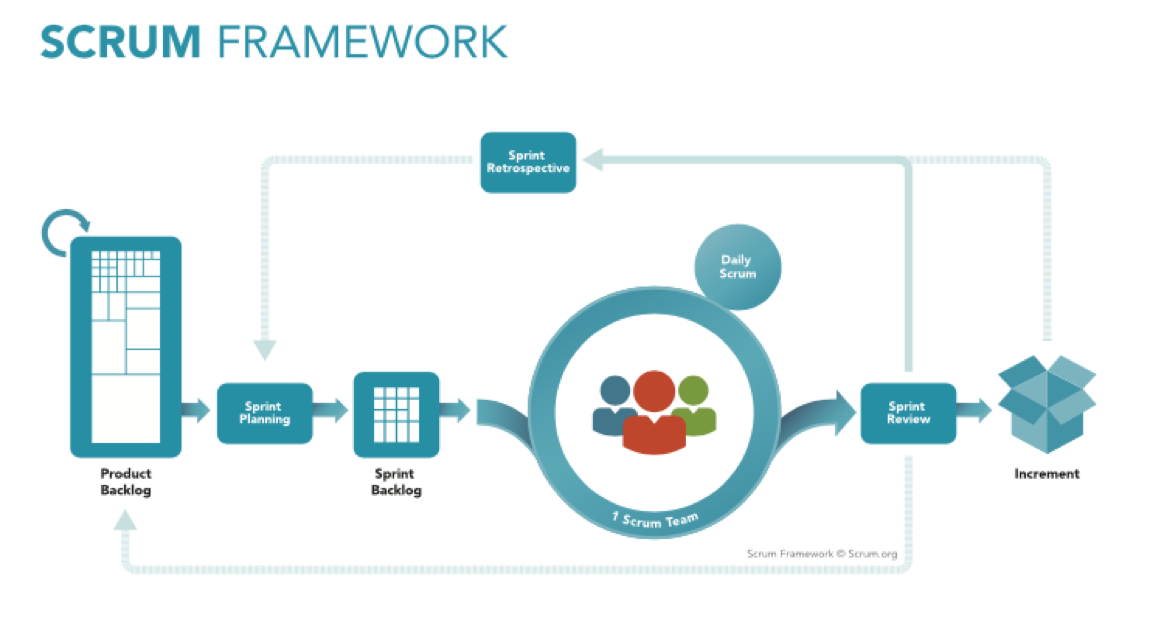
\includegraphics[scale=0.3]{figures/scrum.png}
\caption{Esquema gráfico que explica el funcionamiento de SCRUM.}
\end{center}
\end{figure}
